\documentclass[journal=jpcafh,manuscript=article,layout=onecolumn, 12pt]{achemso}
\usepackage[version=3]{mhchem} % Formula subscripts using \ce{}
\usepackage[T1]{fontenc}       % Use modern font encodings
\usepackage{amsmath}
\usepackage[dvipsnames]{xcolor}
% NB added command for in line cite
\newcommand{\onlinecite}[1]{\hspace{-1 ex} \nocite{#1}\citenum{#1}} 
%
\author{Benjamin~A.~Laws}
\email{b.laws@unsw.edu.au}
\affiliation{School of Chemistry, University of New South Wales, Sydney NSW 2052, Australia}
\alsoaffiliation{Research School of Physics, The Australian
	National University, Canberra ACT 2601, Australia}
\author{Zachariah~D.~Levey} 
\affiliation{School of Chemistry, University of New South Wales, Sydney NSW 2052, Australia}
\author{Timothy~W.~Schmidt} 
\affiliation{School of Chemistry, University of New South Wales, Sydney NSW 2052, Australia}
\author{Stephen~T.~Gibson}
\affiliation{Research School of Physics, The Australian
	National University, Canberra ACT 2601, Australia}
\title{C2H-}
\abbreviations{PES,PAD,EA,eKE,FWHM,VMI}
\begin{document} 
\begin{abstract} 

\end{abstract}
\section{Introduction}
Carbon monohydrides C$_{2n}$H, are a class of linear radicals that play an important role in combustion and interstellar chemistry. These carbon chains have been observed in many interstellar environments, including planetary atmospheres, comets, dark clouds, and during heavy star formation. Due to their relatively high abundance in a variety of astronomical conditions, they have been proposed to be promising candidates for Diffuse Interstellar Band carriers. The corresponding anions C$_{2n}$H$^-$ are also believed to play an important role in interstellar chemistry. C$_6$H$^-$ was the first negative ion detected in space, after it was observed in the circumstellar envelope of IRC+10216 in 2006. More recently, anions C$_4$H$^-$ and C$_8$H$^-$ have also been detected in a range of environments, include dark clouds, prestellar cores, and prostellar envelopes.

Chain growth of the C$_{2n}$H radicals occurs predominately through acetylene addition,
\begin{equation}
\text{C}_{2n}\text{H} + \text{C}_2\text{H}_2 \rightarrow \text{C}_{2n+2}\text{H}+\text{H}_2.
\end{equation}
Conversely, the formation of anions in space is believed to be driven by radiative electron attachment, charge transfer, and dissociate electron attachment. However modelling these processes underestimates the abundance of C$_4$H$^-$ observed in IRC+10216. Therefore, ion-neutral reactions have been proposed as an additional chain growth mechanism that also needs to be considered,
 \begin{equation}
 \text{C}_{2n}\text{H}^- + \text{C}_2\text{H}_2 \rightarrow \text{C}_{2n+2}\text{H}^- + \text{H}_2.
 \end{equation}
Modelling of the extraterrestrial planetary atmosphere of Saturn's moon Titan, suggests that both C$_2$H and C$_2$H$^-$ play an important role in the atmospheric chemistry. Multiple reaction pathways were included for the ion C$_2$H$^-$ including, 
\begin{align}
\text{C}_2\text{H}^- &\xrightarrow[]{\text{H}^+} \text{C}_2\text{H}_2\\
&\xrightarrow[]{\text{HCN}} \text{CN}^-+\text{H}_2\\
&\xrightarrow[]{\text{C}_2\text{H}_2} \text{C}_4\text{H}^-+\text{H}_2\\
&\xrightarrow[]{\text{C}_2\text{H}_2} \text{C}_4^-+\text{H}_3.
\end{align} 

Understanding interstellar chemistry relies critically on theory, to provide a link between astronomical observations and terrestrial laboratory studies. Microwave spectroscopy has successfully been used in this fashion to identify a large number of molecules in the ISM. However for some species, particularly those with low abundances, UV/vis spectroscopic methods are required for identification. This creates a challenge for theory, as electronic spectra calculations are a lot more sensitive to the level of theory employed than pure rotational spectra. This becomes even more challenging when vibronic coupling effects are introduced, as they can be exceedingly difficult to model.

These considerations may be explored by examining some of the smallest carbon monohydrides. The ethynyl radical C$_2$H may appear to be a simple linear triatomic molecule. However the electronic spectrum is complicated by the presence of the close-lying ground $^2\Sigma^+$ and first excited $^2\Pi$ surfaces, which are only separated by $\sim4,000~$cm$^{-1}$. The interaction of these surfaces produces a complex vibronic spectrum around the $\tilde{A}^2\Pi$ origin, where no single band corresponding to the $\tilde{X}-\tilde{A}$ origin has been observed. In C$_4$H the $^2\Sigma^+$ and $^2\Pi$ states are nearly degenerate, resulting in even stronger coupling, while in C$_6$H and C$_8$H the ordering of the states swaps, with a ground $^2\Pi$ state and a low lying excited $^2\Sigma^+$ state. Consequently, understanding these vibronic coupling interactions between the $^2\Sigma$ and $^2\Pi$ surfaces will be essential in order to accurately model the role these radicals (and their corresponding anions) are likely to play in the interstellar chemistry mentioned above, and to discern if they may be possible DIB carriers. 

In this paper we study the vibronic spectrum of the ethynyl radical C$_2$H by employing High-Resolution Photoelectron Imaging (HR-PEI) in order to benchmark CFOUR \emph{ab-initio} vibronic-coupling calculations. C$_2$H is reported to be one of the most abundant molecules in the universe, and is the most thoroughly studied of the C$_{2n}$H species. Many different experimental techniques have been employed to try and resolve the complex vibronic spectrum, including electron spin resonance, laser magnetic resonance, microwave and milli-meter wave spectroscopy, infrared (matrix isolation and Fourier Transform) spectroscopy, and photoelectron spectroscopy. Extensive theoretical work on C$_2$H has also been carried out, in order to try and decode the surprisingly complex spectra that are observed in the experimental studies, however this has proven to be far from straightforward. In this work we demonstrate how the procedures set out in CFOUR may be used to calculate the strength of the vibronic interaction between coupled surfaces near a conical intersection, in order to simulate electronic and vibronic spectra. By employing anion HR-PEI both the $^2\Sigma^+$ and $^2\Pi$ surfaces are mapped out on an equal footing from the anion $\tilde{X}^1\Sigma^+$ state, allowing for direct comparison to the \emph{ab-initio} modelling.

\section{Results and Analysis}
Ethynyl ions were produced in a pulsed-jet discharge of pure C$_2$H$_4$ gas, and subsequently mass isolated via time of flight. Electrons were detached using a tuneable Sunlite Optical Parametric Oscillator (OPO) pumped with the third harmonic of a Nd:YAG laser. High electron counts could also be obtained by using the third and fourth harmonics of the Nd:YAG laser directly. The detached electrons were then mapped onto a micro channel plate detector using a Velocity Map Imaging (VMI) lens. An illustrative VMI of $\sim$4 million electrons collected from 355~nm (3.49~eV) photodetachment of C$_2$H$^-$ is shown in Fig.~\ref{fig:1}(a). The electrons are distributed radially according to their speed, with slow electrons at the image center, and fast electrons located towards the outer edge. Due to the relatively large C$_2$H$^-$ electron affinity (EA) of 2.969~eV~\cite{erv91}, photodetachment at 355~nm occurs close to threshold. This yields slow electrons, allowing for a low repeller voltage ($-600$~V) on the VMI lens, and high velocity resolution. 


Despite being close to threshold, two electronic states of neutral C$_2$H are observed. The faster electrons on the outer edge correspond to C$_2$H$(\tilde{X}\,^2\Sigma^+)+e^- \leftarrow $C$_2$H$^-(\tilde{X}\,^1\Sigma^+)+h\nu$ photodetachment, and are preferentially distributed around the poles of the image, indicative of a positive anisotropy parameter. Conversely the angular distribution of the slower electrons near the center are skewed towards the equator, indicative of a negative anisotropy parameter. These electrons may be assigned to photodetachment to the first excited state C$_2$H$(\tilde{A}\,^2\Pi)+e^- \leftarrow $C$_2$H$^-(\tilde{X}\,^1\Sigma^+)+h\nu$.

\begin{figure}
	
\includegraphics[width=0.8\textwidth]{figures/Fig1}
	\caption{(a) A 3D-representation of the velocity-map image of $\sim$ 4 million photoelectrons detached from C$2$H$^-$ at 355~nm. The outer rings, distributed around the vertical laser polarisation axis, represents photodetachment to the ground $\tilde{X}\,^2\Sigma^+$ state. The inner rings reprsent detachment to the first excited state $\tilde{A}\,^2\Pi$. (b) Photoelectron spectra of C$_2$H$^-$ at a range of detachment wavelengths, illustrating the change in electron intensity profile and energy resolution.}
	\label{fig:1}
\end{figure}

To investigate the vibronic coupling interaction between these two nearby $\Sigma^+$ and $\Pi$ surfaces, deuterated ethynyl C$_2$D$^-$ was also studied. C$_2$D$^-$ ions were produced in a discharge of pure C$_2$D$_4$ gas and measured under the same experimental conditions as C$_2$H$^-$. An illustrative VMI of photodetachment at 355~nm from C$_2$D$^-$ is shown in Fig.~\ref{fig:1}(b). Similarly to Fig~\ref{fig:1}(a) two electronic states are observed - fast electrons with a positive anisotropy corresponding to detachment to the $^2\Sigma^+$ surface, and slow electrons with a negative anisotropy corresponding to $^2\Pi$ detachment. While the fast electrons appear similar in both images, a striking difference is observed in the slow electrons near the detector center. In Fig.~\ref{fig:1}(a) a series of weak rings are observed, however in Fig.~\ref{fig:1}(b) two dominant rings are seen.

The VMI in Fig.~\ref{fig:1} were inverted using the Abel inversion methods detailed in pyAbel, to extract the corresponding photoelectron spectra, which are presented in Fig.~\ref{fig:1}(c). Below $27,000~$cm$^{-1}$ the C$_2$H$^-$ and C$_2$D$^-$ spectra appear very similar. Both are dominated by the origin transition, shifted by $\sim10~$cm$^{-1}$ in the deuterated spectrum, and show a progression in the 2$^{n+1}_0$ and 3$^1_02^{n+1}_0$ vibrational modes. Within the harmonic oscillator approximation, transitions involving an odd quanta of vibrational excitation in the non-symmetric $v_2 (\pi)$ mode should be totally forbidden. However, their presence in the photoelectron spectrum in Fig.~\ref{fig:1}(c) is likely an indicator of Herzberg-Teller (HT) vibronic coupling between the ground $^2\Sigma^+$ and nearby excited $^2\Pi$ electronic surfaces, as
\begin{equation}
\Sigma^+ \otimes \pi = \Pi. 
\end{equation}

Above $27,000~$cm$^{-1}$, near the $\tilde{A}^2\Pi$ state origin, large differences are observed between the C$_2$H$^-$ and C$_2$D$^-$ photoelectron spectra in Fig.~\ref{fig:1}(c). In the C$_2$H$^-$ spectrum 5 sharp peaks are observed, spaced by $\sim95~$cm$^{-1}$. However in the deuterated spectrum, one dominant peak is observed at $27,792$~cm$^{-1}$, with 3 weaker peaks centred around $27,360~$cm$^{-1}$. Unlike the structure below $27,000$~cm$^{-1}$ none of these peaks are able to be readily assigned to vibronic transitions, due to the presence of strong coupling interactions between the nearby $\Sigma^+$ and $\Pi$ surfaces.


%Discuss coupling now...


\subsection{Vibronic Coupling Interactions}
The surprisingly complex spectral structure observed near the $\tilde{A}^2\Pi$ state origin in the photoelectron spectra in Fig.~\ref{fig:1}(c), may be understood by considering the $v_2$ bending vibrational mode. To account for the degeneracy of this mode we may introduce the vibronic quantum number $\ell_i$, representing the angular momentum associated with the bending motion. This may take a value of $\ell_i = v_i, v_i-2, v_i-4,\dots,1$ or $0$, where $v_i$ is the quanta of bending excitation. In the Born-Oppenheimer approximation different vibronic energy levels $\ell_i$ are degenerate, however in cases with strong rovibronic coupling, this degeneracy in $\ell_i$ is lost. 

In C$_2$H this effect creates a Renner-Teller (RT) pair in the excited state, where the usually degenerate $\Pi$ surfaces separate to form two non-degenerate electronic states $\Pi^+ (2A')$ and $\Pi^-(1A'')$. This involves separating a single potential energy surface (V) into two distinct but connected surfaces (V$^+$) and (V$^-$). Due to the strong coupling along the linear axis between the electronic and vibration angular momenta of the $2A'$ and $1A''$ components of the $^2\Pi$ state, stationary states cannot be explicitly assigned to either of the $\Pi^+(2A')$ or $\Pi^-(1A'')$ electronic surfaces. Instead, they exist as a combination of both states.

Due to the close lying nature of the ground {$\tilde{X} ^2\Sigma^+$} and excited {$\tilde{A} ^2\Pi$} electronic states, which are only separated by $\sim3700~$cm$^{-1}$, a pseudo Jahn-Teller effect is also observed. The Jahn-Teller theorem states that stability and degeneracy are not possible simultaneously unless the molecule is linear~\cite{jah37}, meaning that non-linear molecules with degenerate electronic states will undergo a symmetry breaking distortion in order to remove the degeneracy. However a similar effect has also been observed where coupling exists between a non-degenerate state and a nearby pair of degenerate states, even if a molecule is linear.

In the case of ethynyl this is seen as coupling between the ground $\Sigma^+(1A')$ and excited $\Pi^+(2A')$ states, induced by the bending motion of $v_2$. The ground state only couples to one of the Renner-Teller pair $\Pi^+(2A')$, as the other state $\Pi^-(1A'')$ has incorrect symmetry. This results in a very complex vibronic structure for the $\tilde{A}^2\Pi$ electronic state, with contributions from three coupled surfaces $\Sigma^+(1A'),$ $\Pi^+(2A'),$ and $\Pi^-(1A'')$.

These interactions spread the electronic orgin of the $\tilde{A}\,^2\Pi$ state over several vibronic levels. Therefore, instead of assigning a defined origin, the observed peaks in the spectrum may be assigned to coupled admixtures of vibronic transitions involving the three potential energy surfaces,
\begin{equation}
\Psi_f = \sum_\xi \psi_e^\xi \sum_k C_{fk}^\xi\phi_{fkm}^\xi,
\label{eq:teller3} 
\end{equation}
where $\psi_e^\xi$ is the diabatic electronic wavefunction, and $\phi_{fkm}^\xi$ is the spin-rovibrational wavefunction. $\xi$ represents the electronic states used in the expansion, and in this case $\xi=\Sigma^+(1A'),~\Pi^+(2A'),~\Pi^-(1A'')$. A depiction of these three interacting surfaces is given in Fig.~\ref{fig:3}.

\begin{figure}
	\centering
	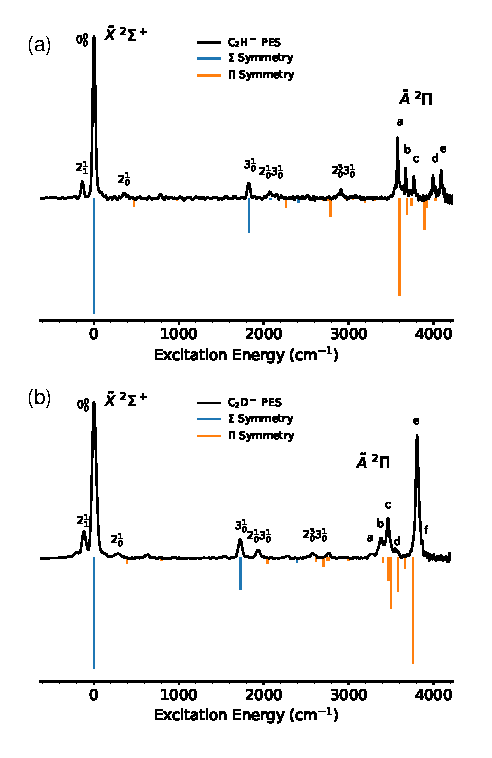
\includegraphics[width=0.5\textwidth]{figures/Fig3}
	\caption{Adiabatic potential energy surfaces of $\tilde{X}^2\Sigma^+$, $\tilde{A}^2\Pi^-$, and $\tilde{A}^2\Pi^+$ states, calculated using the method developed by Tarroni and Carter~\cite{tar03} (E$_{1A'}$, E$_{2A'}$, and E$_{1A''}$ in Eq.~\ref{eq:teller3}).}
	\label{fig:3}
\end{figure}

Tarroni and Carter~\cite{tar03} have demonstrated that a large number of admixed vibronic levels may be calculated using the potential energy surfaces in Fig.~\ref{fig:3}. In fact, over 100 vibronic levels have been calculated, upto 6,400~cm$^{-1}$ above the $\tilde{X}$ state origin. However assigning these levels to experimental spectra has remained a challenge, partly due to the large number of calculated vibronic levels, and partly due to the resolution of the experimental data in the literature. 

%The total number of vibronic levels that need to be considered may be reduced, by examining the symmetry of the level. Conservation of angular momentum dictates only transitions from the anion $\tilde{X}\,^1\Sigma^+$ origin to neutral states with $\Sigma^+$ or $\Pi$ symmetry will be allowed.

\subsection{Photoelectron Angular Distributions}
Symmetry considerations can be employed to help assign the admixed structure in the experimental photoelectron spectra around the $\tilde{A}^2\Pi$ origin. As the detachment laser is linearly polarized, the angular distribution of the electrons in Fig.~\ref{fig:1} may be linked to the symmetry of the detachment orbital. For polarised light, the differential cross section is given by   
\begin{equation}
\frac{\text{d}\sigma}{\text{d}\Omega}=\frac{\sigma_{\text{total}}}{4\pi}[1+\beta P_{2}(\cos\theta)],
\label{eq:beta1}
\end{equation}
where $\theta$ is the angle between the ejected electron and the (vertical) 
laser polarization, and $P_2$ is the second-order Legendre polynomial. The anisotropy parameter $\beta$ provides a quantitative measure of the angular distribution, and can range from -1 to +2 for a pure parallel and perpendicular transition respectively.** From Eq.~(\ref{eq:beta1}), $\beta$ may be determined for each transition in a photoelectron spectrum from the slope of I($\theta$) vs $P_2(\cos\theta)$. Through conservation of angular momentum, it can be shown that $\beta$ may also be expressed in terms of partial waves and dipole matrix elements. Explicitly,
	\begin{equation}
\beta_{\ell} = \frac{[\ell(\ell-1)\chi_{\ell,\ell-1}^2+(\ell+1)(\ell+2)\chi_{\ell,\ell+1}^2-6\ell(\ell+1)\chi_{\ell,\ell-1}\chi_{\ell,\ell+1}\cos\delta_{\ell+1,\ell-1}]/(2\ell+1)}{\ell\chi_{\ell,\ell-1}^2+(\ell+1)\chi_{\ell,\ell+1}^2},
\label{eq:cooper-zare}
\end{equation}
where $\ell$ is the electron orbital angular momentum of the parent anion 
orbital, $\chi_{\ell,\ell\pm1}$ is the radial 
dipole matrix element for the transition from an orbital $\ell$ to 
each of the $\ell\pm1$ partial waves, and $\delta_{\ell+1,\ell-1}$ is 
the phase shift between the two ($\ell\pm1$) partial waves.  

As the radial dipole matrix elements will vary with electron kinetic energy, so too will $\beta$. Therefore, measuring anisotropy parameters at a range of energies will reveal the character of the detachment orbital. Anisotropy parameters were calculated for all resolved transitions in the C$_2$H$^-$ photoelectron spectra from $266-355$~nm, as shown in Fig.~\ref{fig:4}.




Photodetachment to the ground state of C$_2$H$^-$ $(\tilde{X}\,^1\Sigma^+)$ involves ejecting an electron from an $s-$like $5\sigma_g$ orbital, whereas detachment to the excited $(\tilde{A}\,^2\Pi)$ state occurs from a $p-$like $1\pi_u$ orbital.  For a pure $s$ and $p$ orbital, the energy dependence of the anisotropy parameter may be described by Equations (\ref{eq:b-s}) and (\ref{eq:b-p}) respectively,
\begin{equation}
\beta_s = 2,
\label{eq:b-s}
\end{equation}
and,
\begin{equation}
\beta_p = \frac{2\text{A}_1^2\epsilon^2-4\text{A}_1\epsilon\cos\delta_{2,0}}{1+2\text{A}_1^2\epsilon^2},
\label{eq:b-p}
\end{equation}
where the Hanstorp coefficient A$_1$ relates to the ratio of radial matrix elements $\frac{\chi_{1,2}}{\chi_{1,0}}$ and $\delta_{2,0}$ represents the partial wave phase shift. As molecular orbitals may not be pure, we can describe the detachment from C$_2$H$^-$ using the mixed $sp$ model of Sanov~\cite{san14},
\begin{equation}
\beta(\epsilon)_{sp} = \frac{2Z\epsilon+2\text{A}_1\epsilon^2-4\epsilon\cos\delta_{\ell\pm 1}}{\frac{1}{\text{A}_1}+2\text{A}_1\epsilon^2+Z\epsilon}
\label{eq:beta-sanov}
\end{equation}  
where $f$ is the percentage of $p$ character of the orbital,
\begin{equation}
Z = \frac{1-f}{f}\frac{8}{3}~~ \text{and} ~~ |\psi\rangle = \sqrt{1-f}|s\rangle + \sqrt{f}|p\rangle.
\end{equation}

Therefore, calculating the anisotropy parameter for a given transition will reveal the symmetry of the state, which can be compared to the symmetry of the calculated vibronic levels. However this is complicated by the presence of HT coupling, which allows for the electronic character of two surfaces to be mixed via a vibrational promoting mode. As shown in the Supplementary Materials, the transition dipole moment for a HT coupled transition may be rewritten as
\begin{align}
\mu_{\alpha}^{a-n} &= \langle \Psi_{\text{anion}}|\vec{\mu_{\alpha}}|\Psi_{\text{neutral}}\rangle\\
&= \mu_{\alpha:0}^{\tilde{X}-\tilde{X}}\langle\chi_{ms}''|\chi_{jt}'\rangle+\gamma_{kr,jt}\mu_{a:0}^{\tilde{A}-\tilde{X}}\langle\chi_{ms}''|Q_n|\chi_{kr}'\rangle
\label{eq:1}
\end{align}  
where $\mu_{\alpha:0}^{\tilde{X}-\tilde{X}}$ and $\mu_{a:0}^{\tilde{A}-\tilde{X}}$ are the electronic transition moments for the $\tilde{X}\leftarrow\tilde{X}$ and $\tilde{A}\leftarrow\tilde{X}$ transitions, $\chi_{ms}'',~\chi_{jt}',~$and$~\chi_{kr}'$ are the nuclear components of the anion and neutral respectively, and $\gamma_{kr,jt}$ is the vibronic coupling constant. Therefore, HT coupled transitions on the $\tilde{X}^2\Sigma^+$ surface are expected to have anisotropy parameters that reflect the coupled $\tilde{A}^2\Pi$ surface.


Anisotropy parameters were calculated for all strong transitions in the C$_2$H$^-$ photoelectron spectra from $355-266$~nm, as shown in Fig.~\ref{fig:4}. 


%--------------------------------------------
%--Keep this for later (discussion or PAD)---
%--------------------------------------------
HT coupling allows for the electronic character of two surfaces to be mixed via a vibrational promoting mode. As shown in the Supplementary Materials, the transition dipole moment for a HT coupled transition may be rewritten as
\begin{align}
\mu_{\alpha}^{a-n} &= \langle \Psi_{\text{anion}}|\vec{\mu_{\alpha}}|\Psi_{\text{neutral}}\rangle\\
&= \mu_{\alpha:0}^{\tilde{X}-\tilde{X}}\langle\chi_{ms}''|\chi_{jt}'\rangle+\gamma_{kr,jt}\mu_{a:0}^{\tilde{A}-\tilde{X}}\langle\chi_{ms}''|Q_n|\chi_{kr}'\rangle
\label{eq:1}
\end{align}  
where $\mu_{\alpha:0}^{\tilde{X}-\tilde{X}}$ and $\mu_{a:0}^{\tilde{A}-\tilde{X}}$ are the electronic transition moments for the $\tilde{X}\leftarrow\tilde{X}$ and $\tilde{A}\leftarrow\tilde{X}$ transitions, $\chi_{ms}'',~\chi_{jt}',~$and$~\chi_{kr}'$ are the nuclear components of the anion and neutral respectively, and $\gamma_{kr,jt}$ is the vibronic coupling constant. By comparing Eq.~(\ref{eq:1}) to a Taylor series expansion of the transition dipole moment in $Q_n$ about the anion equilibrium geometry, one can see that the vibronic coupling constant may be defined as,
\begin{equation}
\left(\frac{\partial\mu_{\alpha}^{\tilde{X}-\tilde{X}}}{\partial Q_n}\right)_0 = \gamma_{kr,jt}\mu_{a:0}^{\tilde{A}-\tilde{X}}.
\label{eq:2}
\end{equation}
Equation~(\ref{eq:2}) shows that information about the vibronic coupling interaction between the neutral $\tilde{A}-\tilde{X}$ states may be obtained from determining the slope of the $\tilde{X}-\tilde{X}$ electronic transition moment along the vibrational promoting mode coordinate $Q_n$.



%--------------------------------------------------------------------------------
%---------------------------------------------------------------------------------

The resolution attainable using velocity-map imaging is dependent on the energy of the photoelectrons, $\Delta\epsilon\propto\epsilon$. Therefore, measurements close to threshold will provide the highest energy resolution, while shorter wavelength measurements will map a greater extent of the neutral vibrational structure. This variation is illustrated in Fig.~\ref{fig:1}(b), which shows the photoelectron spectra of C$_2$H$^-$ resulting from photodetachment at 266~nm, 300~nm, 310~nm, 320~nm, and 355~nm. In the shorter wavelength measurements, spectral structure related to the $\tilde{A}\,^2\Pi$ state is observed up to 6000~cm$^{-1}$ above the $\tilde{A}$ sate origin. A high resolution photoelectron spectrum of C$_2$H$^-$ detachment at 355~nm extracted from a 2048$\times$2048 image, similar to Fig.~\ref{fig:1}(a), via an inverse Abel transformation, is shown in Fig.~\ref{fig:C2H-355}


 
\section{Conclusions} 

 
\section{Methods}
Details of the HR-PEI spectrometer are given in Refs~\onlinecite{cav07} and~\onlinecite{dev17}. CH$_2$CN$^-$ ions are produced by passing a 1:1 C$_2$H$_4$:N$_2$O gas mixture through a pulse valve, which then undergoes supersonic expansion into a high-voltage discharge. Negative ions are extracted, accelerated to 500~eV, and focussed into a novel gating, bunching, and re-referencing unit~\cite{ded01}. Anions are mass separated over a 2m time-of-flight region, with the ion of interest isolated by an electrostatic gate. The ion packet is crossed with a tuneable detachment laser beam, generated from a Sunlite EX optical parametric oscillator pumped by the third harmonic of a Continuum Powerlite 9010 Nd:YAG laser. The laser produces between 10-50mJ per pulse at 10Hz, depending on whether the idler or signal beam is used. The wavelength of the laser light is measured using a HighFinesse WS7 UV wavemeter.

A velocity-map imaging lens, a modified version of the original concept of Eppink and Parker, images the detached electrons to a 75mm diameter MCP/phosphor screen detector. Events are imaged by a 2014x2048 monochrome CCD camera (PCO 2000), with each frame transferred to a computer at a 10Hz repetition rate, and processed in real time to identify individual electron events. The electron positions are centroided to a sub-pixel accuracy, then written to a data file for subsequent analysis. The velocity-map image is centred and then circularized by an angular dependent-radial scaling determined by comparing adjacent radial slice intensity profiles~\cite{gas17}. An inverse Abel transformation of the VMI, based on the algorithm of Hansen and Law~\cite{han85,pya16}, returns a slice image of the 3D electron source distribution. Absolute energy calibration of the photoelectron spectra is achieved using published measurements of species, including O$^-$~\cite{cav07} and NO$_2^-$~\cite{law19}, that have been studied under similar conditions as used for the CH$_2$CN$^-$ measurements.

In standard operation, the energy distribution of the detached electrons is obtained by recording the velocity-mapped positions from photodetachment at a fixed wavelength. However the HR-PEI spectrometer may also be reconfigured into an electron counting mode, where the number of events per laser shot is recorded, while the detachment laser wavelength is varied.







%Hi~\cite{law17}

\begin{acknowledgement}
	This research was supported by the Australian Research Council Discovery
	Project Grants DP160102585 and DP190103151.  
\end{acknowledgement}

% Create the reference section using BibTeX: 
\bibliography{C2H.bib}

\end{document}
% ****** End of file apstemplate.tex ******